\documentclass{report}
\usepackage{indentfirst}
\usepackage{graphicx}
\usepackage{float}
\graphicspath{ {./Imagens/} }

\setlength{\parindent}{4em}
\setlength{\parskip}{0.5em}

\begin{document}

\title{\Huge{\textbf{FEUPBook}} \\ Relatório BDAD 2019/2020 \\ \Large{2MIEIC04}}
\author{Eduardo Correia \\ \texttt{up201806433} \and
	    Ricardo Fontão \\  \texttt{up201806s317} \and
        João Diogo \\ \texttt{up201806779}}
\date{\today}

\begin{figure}[b] % Bottom of page
    \centering
    
\includegraphics[width=0.8\textwidth]{feup-logo}
\end{figure}

\maketitle

\tableofcontents

\chapter{Introdução}

O nosso projeto consiste numa rede social denominada \textit{FEUPBook} (inspirado pela já existente rede socal,  \textit{Facebook}). Nesta, utilizadores poderão criar uma conta pessoal para falar uns com os outros e ver diversas publicações do seu interesse no seu \textit{feed}.

\chapter{Especificação} 

\section{Multimédia}

A rede social do nosso projeto possui a capacidade de partilhar ficheiros multimédia, quer seja através de mensagens ou publicações e dividem-se essencialmente em três categorias, áudio, imagem e vídeo. Cada ficheiro destes possui um \underline{título}, correspondente ao seu nome em memória, bem como um \underline{url} que indica a localização do ficheiro para lhe aceder. \par

TODO: Limite do tamanho de ficheiros. É possível enviar ficheiros binários (?)

\subsection{Áudio}

Este tipo de ficheiro é nomeadamente 

.mp3 .wav (?)

\subsection{Foto}

.jpg .png .bmp (?)

\subsection{Vídeo}

\section{Utilizador}

Esta classe representa um membro da rede social. Este possui um nome e id único para o identificar (correspondente ao último campo do \textit{url} do seu perfil). \par

Um utilizador, por norma, terá diversas amizades com outros, para que possa aceder aos conteúdos do seu perfil, conversar mais facilmente com ele e ver as publicações no seu feed. Para esse efeito, terá de enviar um pedido de amizade ao outro, o qual pode ser aceite ou não.

\section{Página}

\section{Publicação}

\section{Comentário}

\section{Reação}

\section{Grupo}

Um grupo possui como função agregar diversos utilizadores que queiram estar juntos por

\section{Conversa}

Numa rede social é indispensável a capacidade de os utilizadores conversarem entre si, como tal estes podem agregar-se numa \underline{conversa} (que possui no mínimo 2 utilizadores). \par

Uma conversa é composta por diversas \underline{mensagens}

Ainda no contexto de uma conversa, cada utilizador pode possuir uma \underline{alcunha} própria.

\section{Mensagem}

Uma mensagem é o modo como os utilizadores comunicam numa \underline{conversa} e como tal possuir um \underline{texto} associado, que corresponde ao que o utilizador pretende dizer. No entanto, este \underline{texto} pode ser uma \textit{empty string}.

\section{Evento}

Se um utilizador desejar, pode criar um evento para marcar um acontecimento relevante e convidar outros utilizadores a participarem no mesmo. \par

Um evento possui um nome que o identifica, bem como uma breve descrição do que se trata, o local em que vai ocorrer e a sua data da sua realização.

\chapter{Modelo concetual}

\begin{figure}[H]
    \centering
    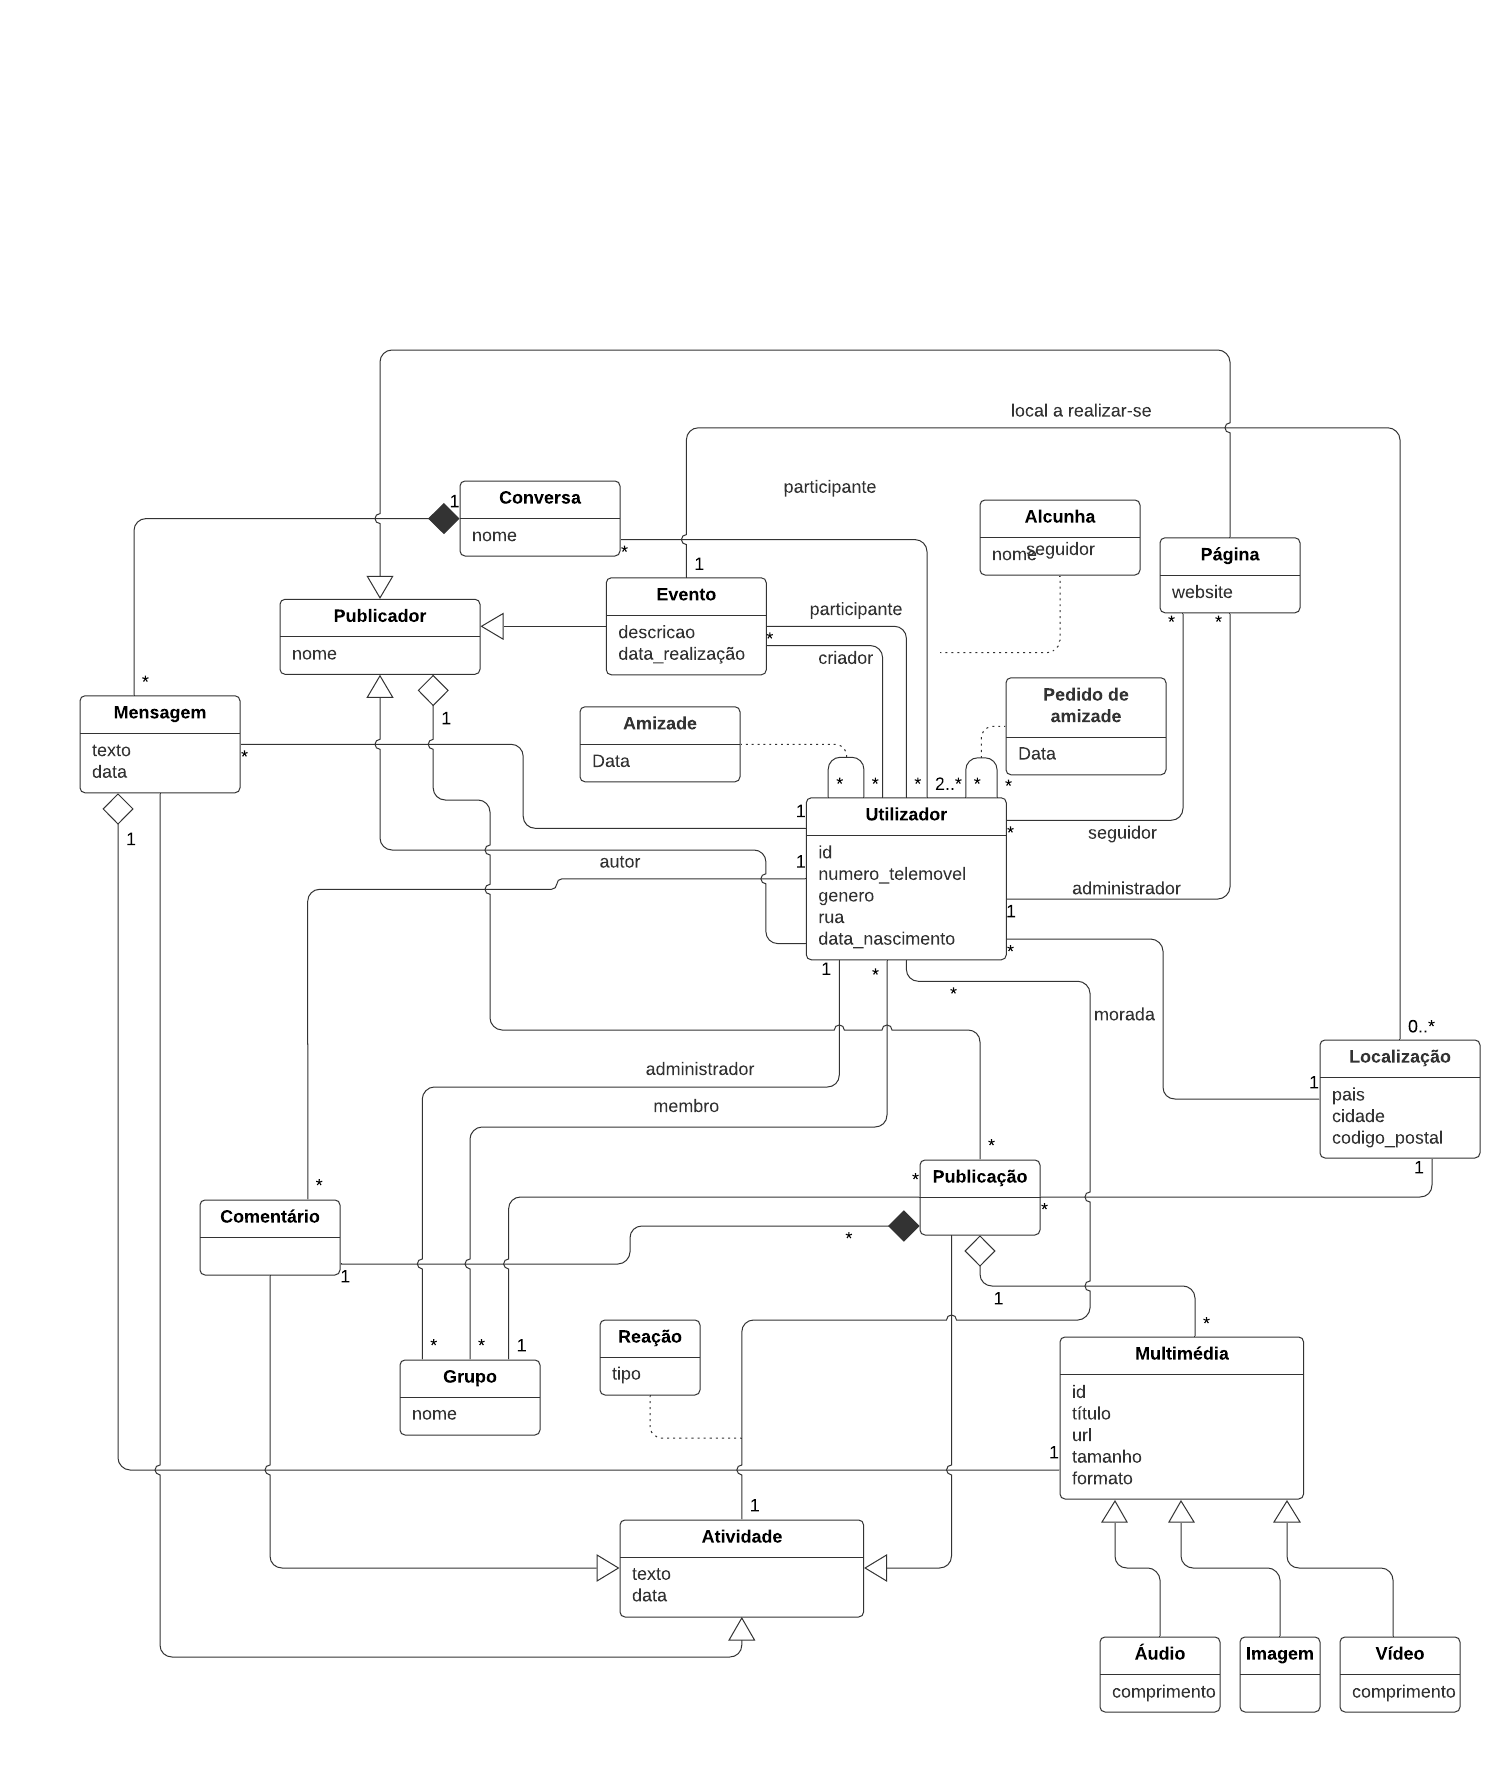
\includegraphics[width=\textwidth]{diagram}
\end{figure}

\end{document}